In this section will be presented an overview of the user’s interface of the CKB platform.
The focus will be mainly on the user experience. 
\verb|CKB| is accessible using any browser and does not have a client application.
Images shown below depicting the user interface include both samples for the desktop browser version and the mobile version.

\section{General Overview}
\label{sec: general_overview}%
The image below shows a map of the pages which can be accessed from the web application.
All pages are available after the user has logged in, except for the registration page and the login page itself.

\begin{figure} [H]
    \begin{center}
        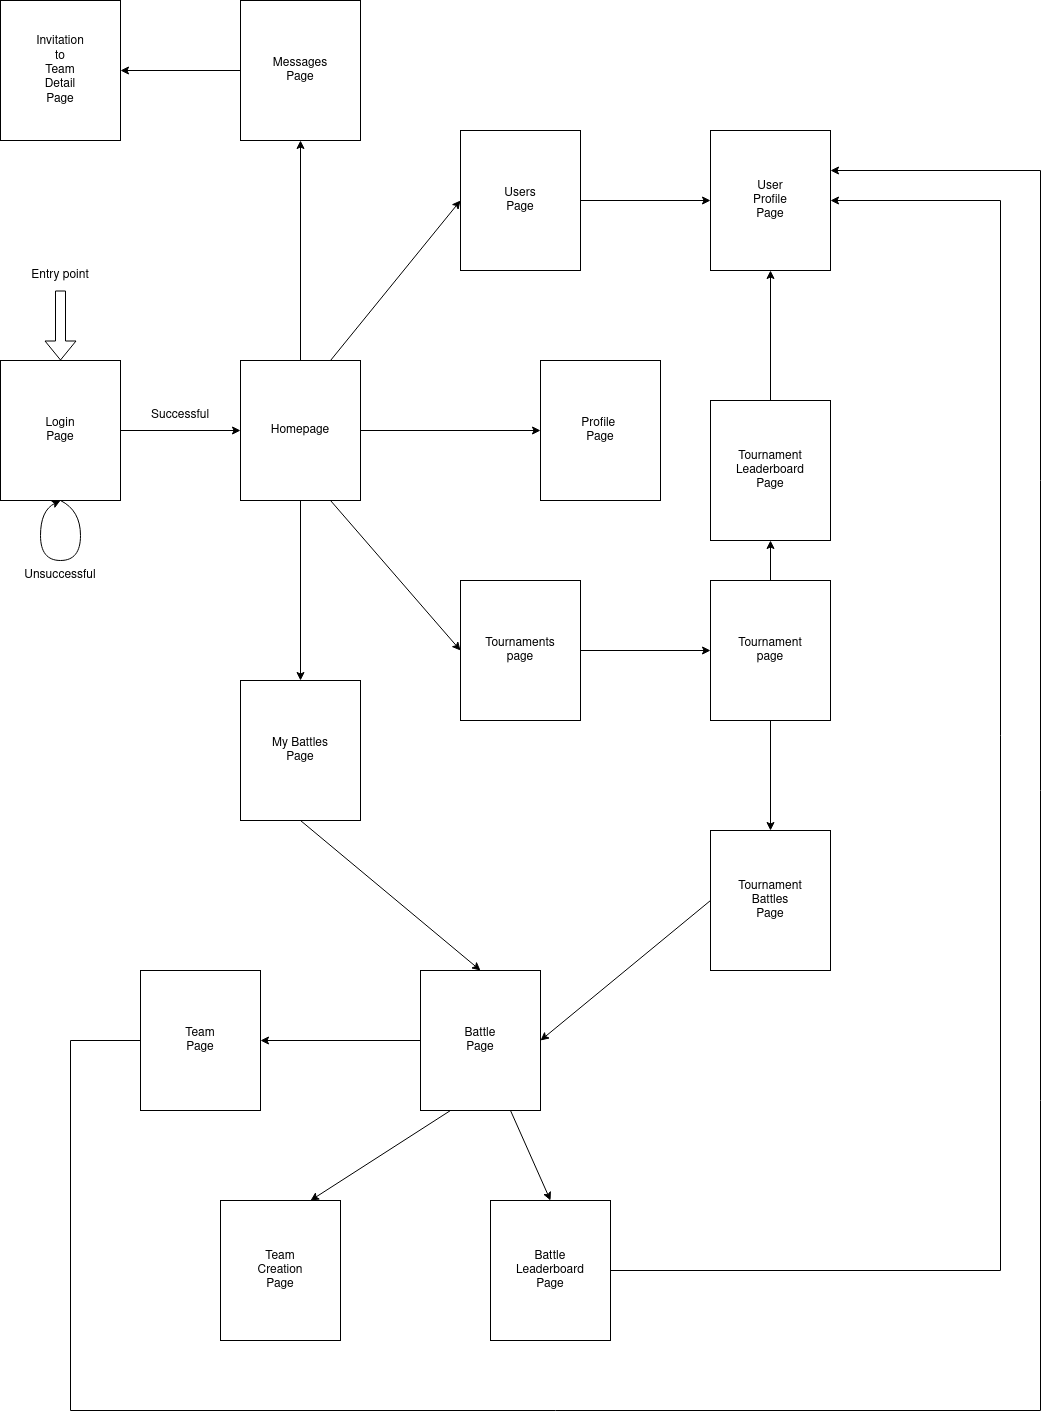
\includegraphics[width=1\linewidth]{Images/designmap.png}
        \caption{Pages of the CKB platform}
        \label{fig: designmap}
    \end{center}
\end{figure}

The login page prompts the user to enter their institution email and redirects them to the login page of their institution, 
which is not part of the CKB platform so it is not shown here.
A successful login (validated by the institution) will redirect the user to the homepage of the CKB platform, which will differ depending on the role of the user.


\section{Registration, Login and Homepage}
\label{sec: registration_login_homepage}%
The following mockups show the SignUp page and the LogIn page. 
Depending on the type of user, the Homepage will be slightly different, as Educators will have a menu entry allowing them to
create new Tournaments or CodeKataBattles directly from the Homepage.

\begin{figure}[H]
    \begin{minipage}{0.45\linewidth}
        \centering
        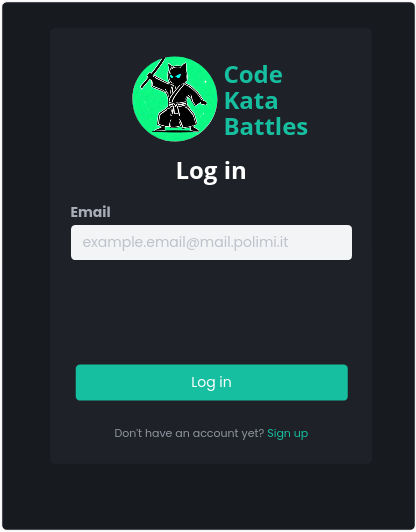
\includegraphics[width=\linewidth]{design/login.png}
        \caption{CKB Log in page}
        \label{fig: login}
    \end{minipage}\hfill
    \begin{minipage}{0.45\linewidth}
        \centering
        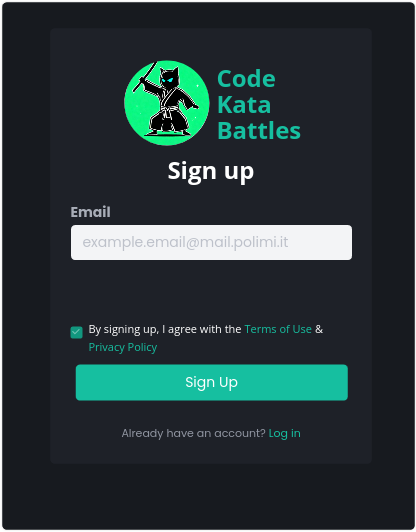
\includegraphics[width=\linewidth]{design/signup.png}
        \caption{CKB Sign Up page}
        \label{fig: signup}
    \end{minipage}
\end{figure}

Both the SignUp page and the LogIn page will redirect the user to the institution's login page as anticipated in Section \ref{sec: general_overview}.
\newpage
\section{Homepage}
\label{sec: homepage}%
The Homepage is the first page the user will see after logging in. 

\begin{figure} [H]
    \begin{center}
        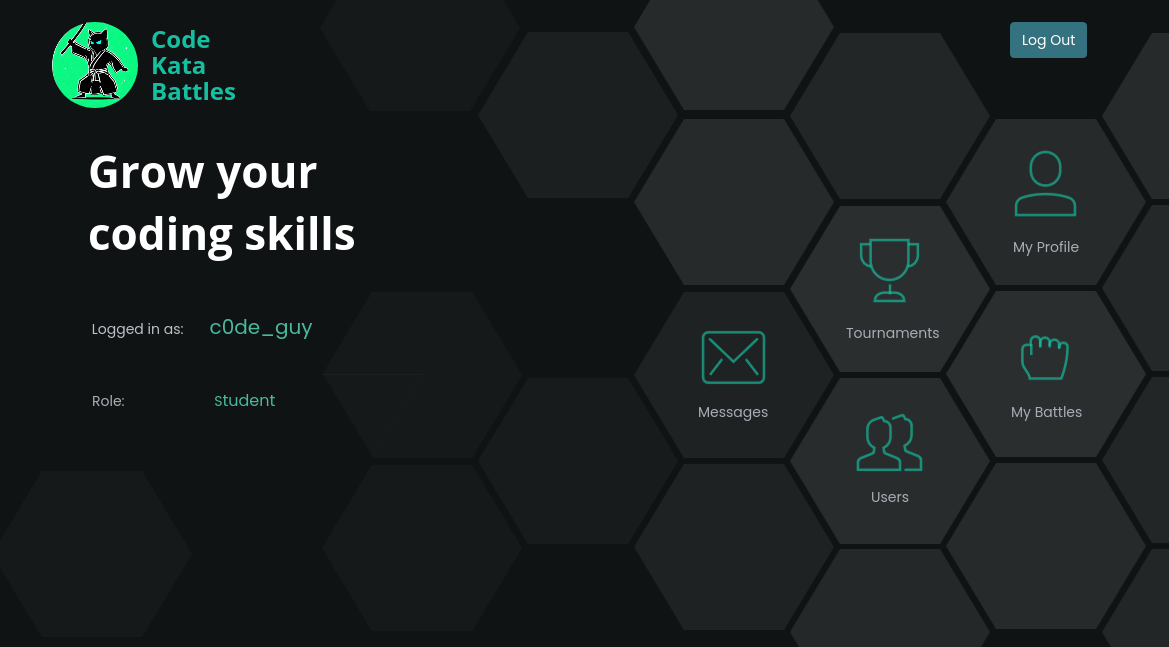
\includegraphics[width=1\linewidth]{design/student_homepage.png}
        \caption{CKB Student Homepage}
        \label{fig: student_homepage}
    \end{center}
\end{figure}
The Student Homepage (Figure \ref{fig: student_homepage}) will show a LogOut button, and 5 menu options:
\begin{itemize}
    \item \textbf{My Profile}: this will redirect the user to their profile page.
    \item \textbf{Tournaments}: this page will show the list of all the tournaments available and the ones the user is currently enrolled in.
    \item \textbf{My Battles}: this page will show the list of all the CodeKataBattles the user is currently enrolled in. This allows the student to 
    jump directly to the page of a battle without having to go through the tournament page.
    \item \textbf{Users}: this page will show the list of all the Students enrolled in the platform. 
    Selecting a user from the list in this page opens the profile page of the selected user, showing Badges earned.
    \item \textbf{Messages}: this page will show the list of all the messages received by the user, including Team Invitations and notifications about new Tournaments or Battles or the end of them.
\end{itemize}

\begin{figure} [H]
    \begin{center}
        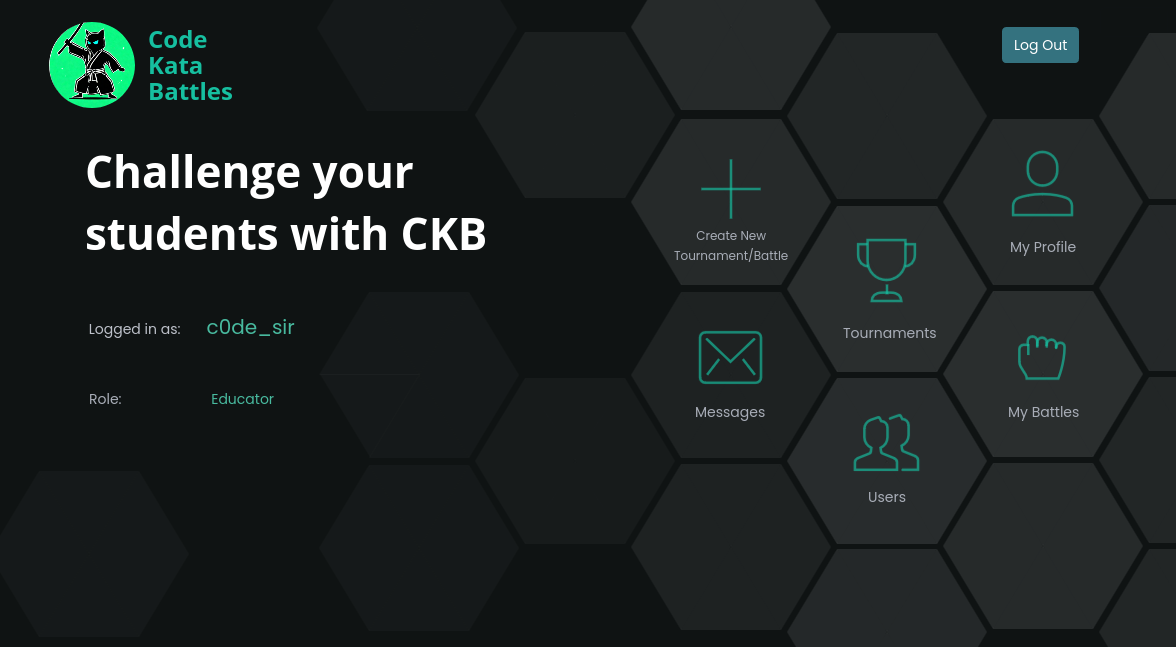
\includegraphics[width=1\linewidth]{design/educator_homepage.png}
        \caption{CKB Educator Homepage}
        \label{fig: educator_homepage}
    \end{center}
\end{figure}

The Educator Homepage (Figure \ref{fig: educator_homepage}) will show a LogOut button, and 6 menu options:
\begin{itemize}
    \item \textbf{My Profile}: this will redirect the user to their profile page.
    \item \textbf{Tournaments}: this page will show the list of all the tournaments available.
    \item \textbf{My Battles}: this page will show the list of all the CodeKataBattles the Educator is currently administrating. This allows the educator to 
    jump directly to the page of a battle without having to go through the tournament page.
    \item \textbf{Users}: this page will show the list of all the Students enrolled in the platform. 
    Selecting a user from the list in this page opens the profile page of the selected user, showing Badges earned.
    \item \textbf{Messages}: this page will show the list of all the messages received by the user, including the start of a Battle administrated by the Educator. 
    \item \textbf{Create new Tournament/Battle}: this page will allow the Educator to create a new Tournament/Battle.
\end{itemize}

\newpage
\section{Profile Page}
\label{sec: profile_page}%
After SignUp  the user will be redirected to the Profile Creation page (Figure \ref{fig: profilecreation}), 
where they will be asked to provide a unique personal username to be used in the \verb|CKB| platform.
\begin{figure} [H]
    \begin{center}
        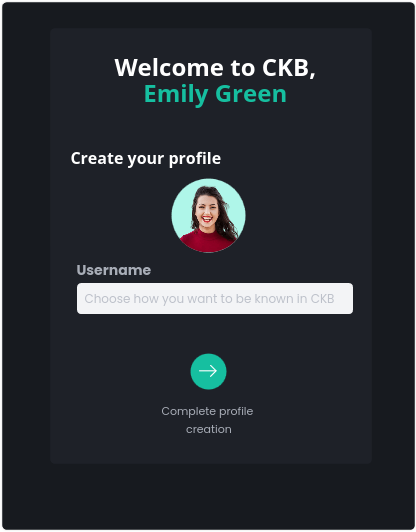
\includegraphics[width=0.45\linewidth]{design/profilecreation.png}
        \caption{Profile creation page}
        \label{fig: profilecreation}
    \end{center}
\end{figure}

The Profile Page (Figure \ref{fig: prof_page}) will show the user's profile picture, the username, their real name and surname and the list of Badges earned.
Clicking on a Badge will open a popup with a description of the Badge, describing how it was achieved.
\begin{figure} [H]
    \begin{center}
        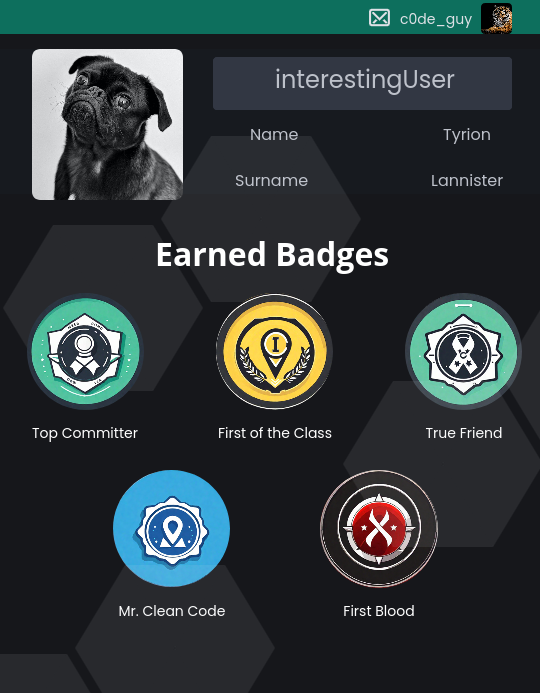
\includegraphics[width=0.5\linewidth]{design/profile_page.png}
        \caption{CKB profile page}
        \label{fig: prof_page}
    \end{center}
\end{figure}






\section{Tournaments and Battles}
\label{sec: tournaments_battles}%
Tournaments and Battles pages are simply a list of all the Tournaments/Battles available. 
Clicking on a Tournament/Battle will open the Tournament/Battle page. No mockups are provided for these pages as they are very simple.

\subsection{Leaderboards}
\label{subsec: leaderboards}%
\begin{figure} [H]
    \begin{center}
        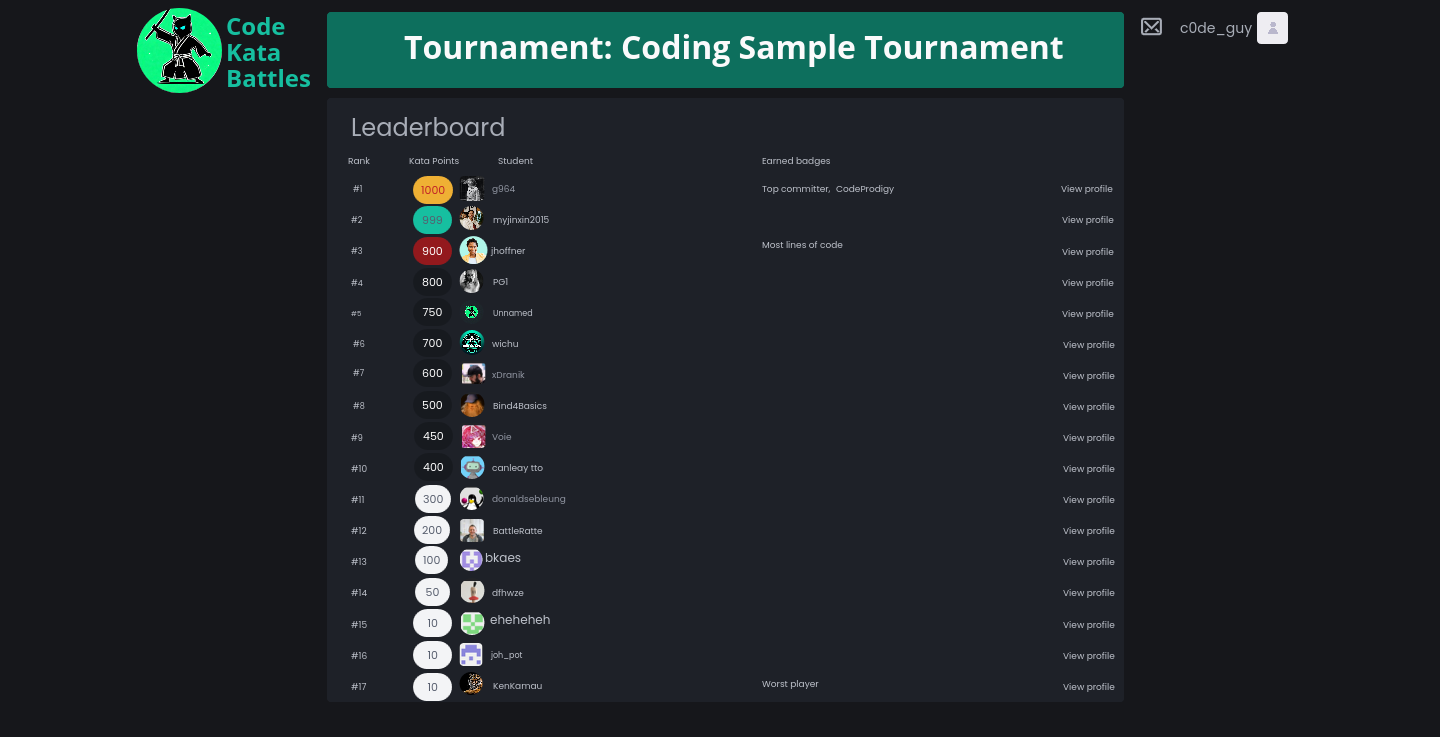
\includegraphics[width=1\linewidth]{design/tournament_leaderboard.png}
        \caption{Tournament leaderboard page}
        \label{fig: tournament_leaderboard}
    \end{center}
\end{figure}
The Tournament Leaderboard page (Figure \ref{fig: tournament_leaderboard}) will show the ranking of all the students enrolled in the tournament, in descending order.
The Students who earned more points appear upper in the list. 
The points are calculated as the sum of the points earned in each battle of the tournament.
Each row of the leaderboard will show a Student's ranking (position), their score, their username, the badges they earned in the tournament (if any) and a button to view their profile.
Clicking on 'View Profile' will open the profile page of the selected user.

\begin{figure} [H]
    \begin{center}
        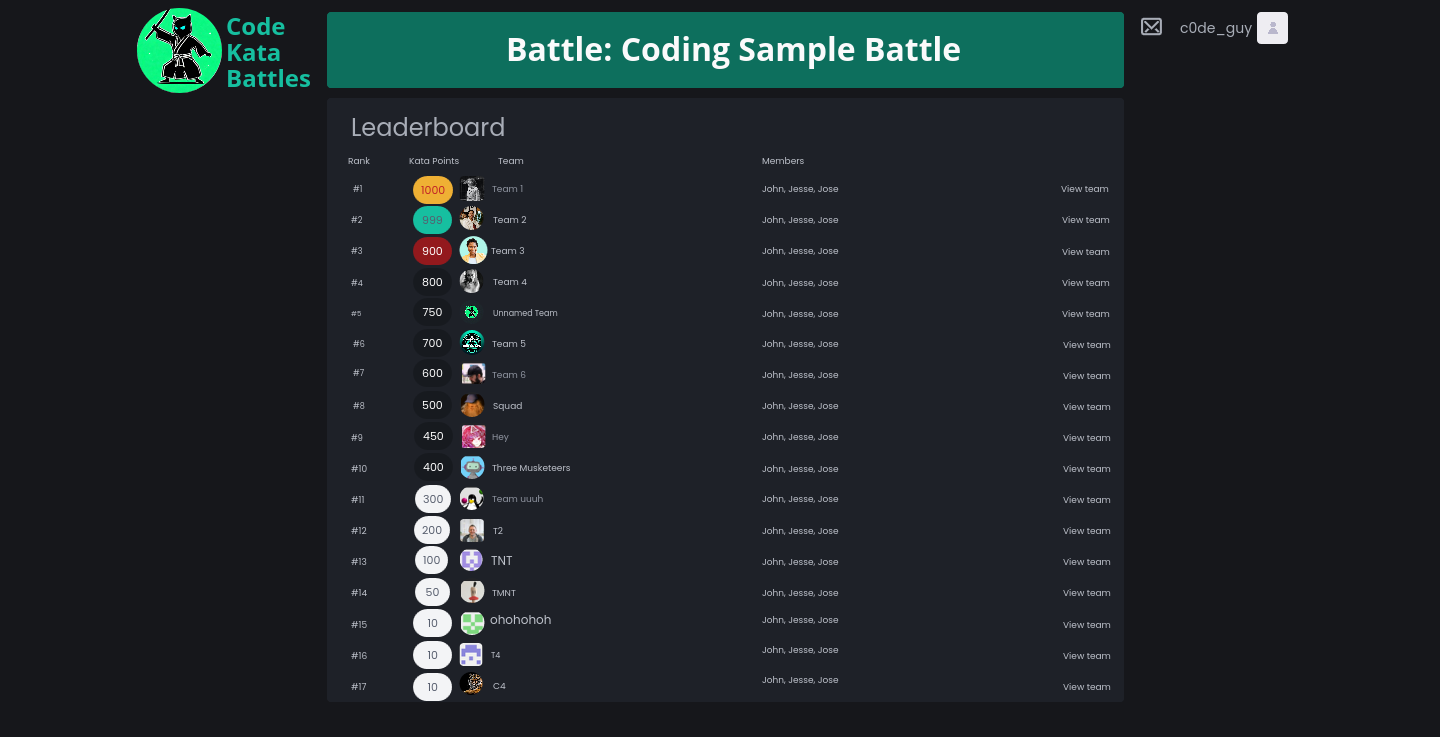
\includegraphics[width=1\linewidth]{design/battle_leaderboard.png}
        \caption{Battle leaderboard page}
        \label{fig: battle_leaderboard}
    \end{center}
\end{figure}
The Battle Leaderboard page (Figure \ref{fig: battle_leaderboard}) will show the ranking of all the Teams enrolled in the battle, in descending order.
The Teams who earned more points appear upper in the list.
Each row of the leaderboard will show a Team's ranking (position), their score, their name, the usernames of the members of the team and a button to view the Team Page.
Clicking on 'View Team' will open the Team page of the selected team.
No mockups are provided for the Team page as it is very simple: a list of the members of the team along with the public info of the members.


\subsection*{Battle Page from both Educators and Students' perspective}
\label{subsec: battle_page}%
The \verb|Battle Page| will be different depending on the role of the user.

A Student will see the description of the battle, the link of the GitHub repository they are supposed to work on, the list of the other Teams enrolled in the battle,
 the username of the Educator who created the battle, the submission deadline for solutions and the registration deadline.
In case the Battle has already started, the list of Teams participating will be replaced by the leaderboard of the Battle.
The GitHub link will be visible only after the Battle starts.
A sidebar on the right shows the Students belonging to the Team of the logged in user.
In case the user and their team are not enrolled in the Battle, the sidebar will show a button to enroll in the Battle and a button to invite other Students to join the Team.
Minimum and maximum Team capacity are shown in the sidebar.
If the team is composed of less than the minimum number of students, the \verb|Join Battle| button will be disabled.
If the team is composed of the maximum number of students, the \verb|Invite more| button will be disabled.
\begin{figure} [H]
    \begin{center}
        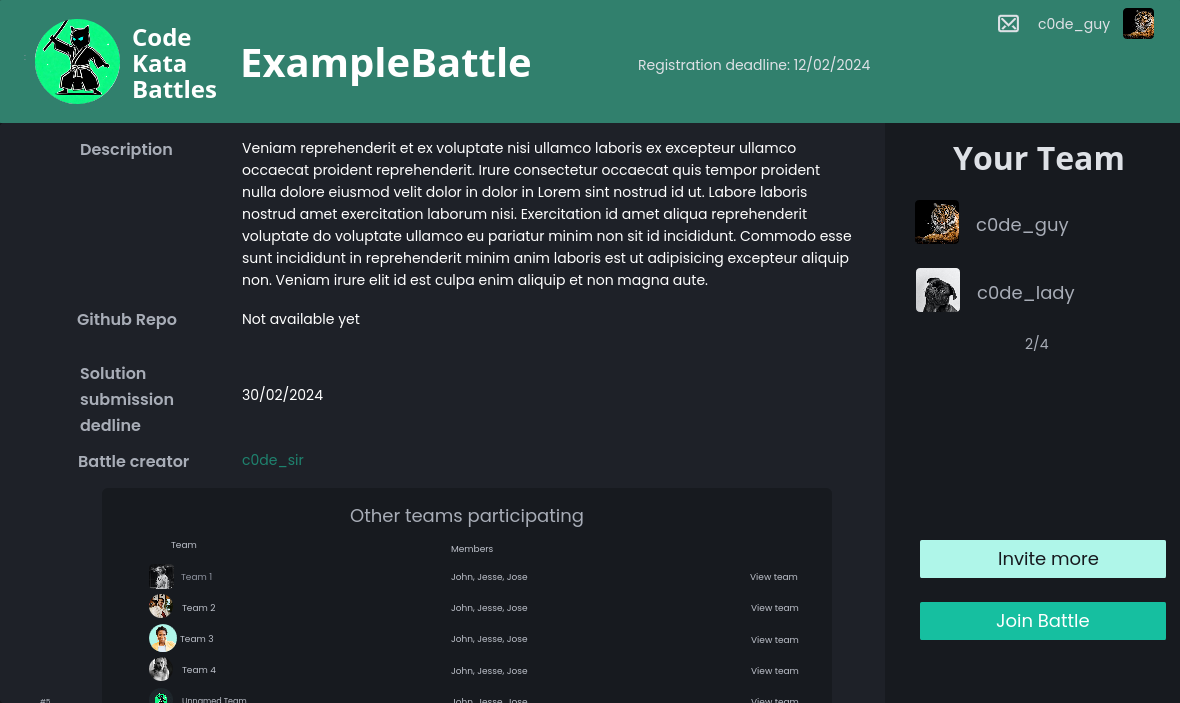
\includegraphics[width=1\linewidth]{design/battle_page_student.png}
        \caption{Battle page for student}
        \label{fig: battle_page_student}
    \end{center}
\end{figure}


An Educator will see the all the info shown to the Students except for the sidebar.
The Educator, after the end of the Battle, will be able to evaluate the solutions submitted by the Teams.
The evaluation page is shown in Figure \ref{fig: battle_eval}.
An initial score is assigned to each Team (calculated by the automated evaluation system), which can be modified by the Educator. 
The Leaderboard shows for each row:
\begin{itemize}
    \item the Team's ranking (position)
    \item the Team's score
    \item the Team's name
    \item the usernames of the members of the team
    \item the score automatically assigned by the system regarding the Functional Aspects of the solution
    \item the score automatically assigned by the system regarding the Timeliness (submission time) of the solution
    \item the score automatically assigned by the system regarding the Quality of Code aspects of the solution
    \item a button to manually modify the Team's score examining their solution
\end{itemize}
A button \verb|Finalize Evaluation| allows the Educator to finalize the evaluation of the Battle and make the results available to everyone.
\begin{figure} [H]
    \begin{center}
        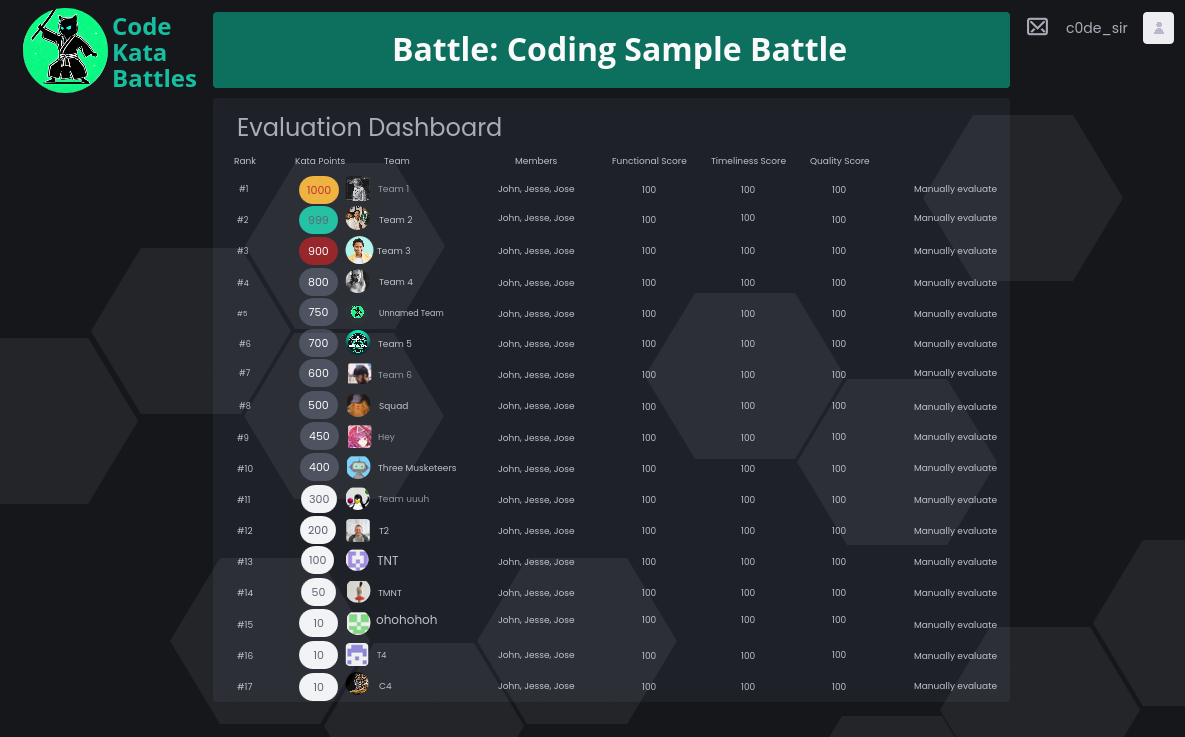
\includegraphics[width=1\linewidth]{design/battle_evaluation.png}
        \caption{CKB Battle Evaluation Dashboard}
        \label{fig: battle_eval}
    \end{center}
\end{figure}




\section{Teams and Invitations}
\label{sec: teams_invitations}%

Clicking on the \verb|Invite more| button in the Battle page (Figure \ref{fig: battle_page_student}) will open the \verb|Invite other Students| page (Figure \ref{fig: invite_others}).
The page will show a list of all the Students enrolled in the Tournament the Battle belongs to who are not already enrolled in the Battle with a Team. 
The user can select one or more Students from the list and click on the \verb|Invite| button to send them an invitation to join the Team. 
The list of Students show their username, their email and the state of the invitation (Refused/Free/Joined/Pending).
Clicking on the \verb|Invite| button will send invitations to the selected Students.
\begin{figure} [H]
    \begin{center}
        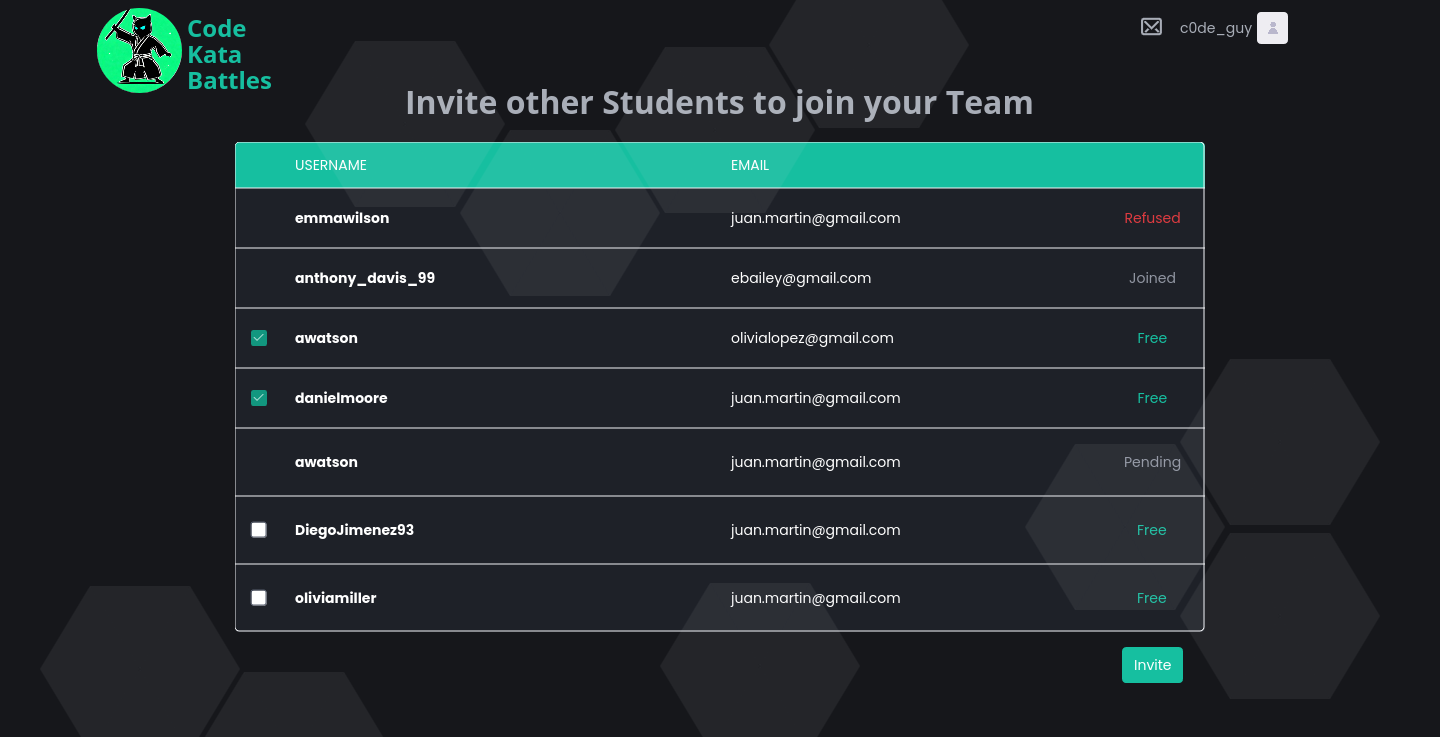
\includegraphics[width=1\linewidth]{design/invite_other_students.png}
        \caption{Invite other students page}
        \label{fig: invite_others}
    \end{center}
\end{figure}


A Student who receives an invitation will see a notification in the \verb|Messages| page.
Opening the notification will show the invitation popup (Figure \ref{fig: invitation_popup}).
The popup will show the name of the Student that sent the invitation, the name of the Battle.
Clicking on the name of the Battle will open the Battle page, allowing the user to develop an informed decision about accepting or refusing the invitation.
Clicking on the \verb|Accept| button will enroll the user in the Battle with the Team that sent the invitation.
Clicking on the \verb|Decline| button will refuse the invitation.
\begin{figure} [H]
    \begin{center}
        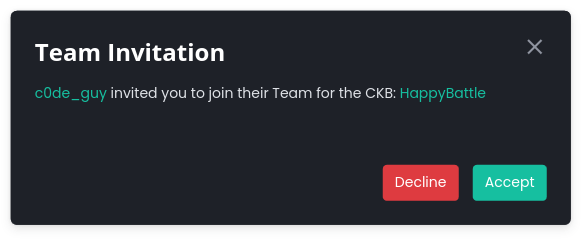
\includegraphics[width=0.7\linewidth]{design/invitation_popup.png}
        \caption{Invitation popup}
        \label{fig: invitation_popup}
    \end{center}
\end{figure}









